\section{Approaches to incorporate WordNet information}\label{sec:approaches_ext_res}
Having the dataset of the previous section, we next try to improve our latest re-implementation Residual-Stacked Encoder\textsuperscript{$\dagger$} using WordNet. 
\subsection{Methods}
Unlike \ac{KIM}, which has shown an intuitive and successful strategy of incorporating WordNet, the Residual-Stacked Encoder does not use inter-sentence attention. Without changing this, we therefore cannot likewise align words of $p$ with words of $h$ to identify their WordNet relation. We intend to leave the model with the plain sentence-encoding architecture, targeting the incorporation of external resources for general sentence representations, encoding each sentence individually \citep{nangia2017repeval}. Naturally, this poses a new difficulty, since the relations of WordNet are defined between two senses. Subsequentially, we apply other strategies, than directly encoding the relation of two words (or senses), explained below.
\subsubsection{Drawbacks of using insights of max-pooled sentence representations}
In Section §\ref{sec:understanding} we gained valid insights on the sentence-representations, and showed that these sucessfully can be used to change the meaning of sentence representations. Following these conclusions, a possible strategy is, to train the model in a way, that antonyms or co-hyponyms result in distinct high dimensions, synonyms in the same high dimensions and hypernyms in a subset of high dimensions compared to hyponyms. Knowing reasonable values for each values within the dimensions, this could be broken down to a simple regression problem. Since we did not find an elegant way to naturally include this into the loss function, the only remaining strategies highly reassemble traditional feature-engineering, as the $\xi$ would need to be determined beforehand. Since the automatic feature selection is one of the key strengths of neural models \citep{bengio2013representation}, those strategies would rather be similar to a step backward than forward. Instead we identify to potential strategies, that are simpler to implement and would result in a broader applicability, not being tied to max-pooled sentence representations.

\subsubsection{Fuse WordNet information within the embedding-layer}
Additional information within the word-representations has the advantage, of being generally applicable. Following \cite{ruckle2018concatenated} we do not use exclusively retrained or adjusted word-embeddings. Instead, for each word $w$ we look up the word-vector within the original distributed GloVe embeddings and concatenate it with the corresponding word-vector of the same $w$ from the additional word-embeddings. If no vector for $w$ is present within those, we concatenate a zero-valued vector of the same dimensionality. Thus, we do not limit the original information of distributed word-embeddings and the model may still rely on the same features. Even though some of the additional features might be redundant w.r.t. the orignal GloVe embeddings, some contain additional information, that the network can use to differentiate between words, that are highly similar in GloVe. Additional to doing this experiment with the mono-lingual attract-repel vectors, provided by \cite{ruckle2018concatenated}, we use two different word-vector sources.

\paragraph*{Overfitting WordNet}
We apply a simple method to create addtitional word vectors $v$ that are similar for the words $w_1$ and $w_2$, if they are synonyms, and distinct if $w_1$ and $w_2$ are antonyms or co-hyponyms. For this we extract samples ($w_1$, $w_2$, \texttt{relation}), whereas $w_1$ and $w_2$ are lemmata, that are linked via \texttt{relation} within WordNet, represented by their GloVe embeddings. Using a two layer \ac{MLP}, we map each word-vector $w \in \mathbb{R}^{300}$ to $v \in \mathbb{R}^{20}$. In our last layer we apply $\tanh$ as non-linearity, to squeeze all values $v^i$ within $v$, with $v^i$ being the $i$th value within $v$, are in an appropriate range:  $ \forall i: [i \in \{x \in \mathbb{N} | x < 20\} \Rightarrow v^i \in \{x \in \mathbb{R} | -1 < x < 1\}]$. Let $w \in \mathbb{R}^{300 \times 1}$ be the GloVe word-embedding, $W_1 \in \mathbb{R}^{100 \times 300}$ and $b_1 \in \mathbb{R}^{100 \times 1}$ the weight matrix and bias of the first layer, and $W_2 \in \mathbb{R}^{20 \times 100}$ and $b_2 \in \mathbb{R}^{20 \times 1}$ of the second layer respectively. The new word-vector $v$ is calculated as:
\begin{equation}
v = \tanh(W_2 \text{ reLU}(W_1w + b_1) + b_2)
\end{equation}
We optimize the representations $v_1$ and $v_2$, coming from ($w_1$, $w_2$, \texttt{relation}) using \ac{MSE} with the Eucledian Distance, which should be high, if the relation indicates, $w_1$ and $w_2$ are mutually exclusive, and low, if both are synonyms. We define $\theta=0$ for synonyms, and $\theta =10$, for antonyms and co-hyponyms respectively (we bound the difference to $\frac{|v|}{2}$, with $|v|$ being the amount of dimensions of the new word-vectors, as it creates sufficiently distinct vectors) and calculate the loss as:
\begin{equation}\label{eq:loss_embd}
\text{loss} = \frac{1}{2}\Bigg( \sqrt{\sum^{20}_{i=1}(v^i_1 - v^i_2)^2} - \theta\Bigg)^2
\end{equation}
We overfit on the lexical relations extracted from WordNet, intending to memorize whether two words are compatible or not. This optimization process also updates the GloVe embeddings of $w$ during training. In order to create word-vectors that specifically focus on either antonymy or co-hyponomy, we train embeddings for each of those relations individually, both times together with synonyms in order to have a counterpart. Embeddings differentiating between synonyms and antonyms are referred to as \textit{Trained-Syn-Ant}, differentiation between synonyms and co-hyponyms as \textit{Trained-Syn-Cohyp}. We refer to the concatenation of both embeddings as \textit{Trained-Syn-Cohyp-Ant}. Since the Eucledian Distance is a symmetric measure we cannot include the hypernym-hyponym relation into those embeddings. We thus train other embeddings, differentiation between all relevant lexical semantic relations\footnote{Synonymy, Antonomy, Hypernyomy, Co-hyponomy} in a slightly adapted manner, and with 50 instead of 20 dimensions. In order to enable the network to deal with asymmetric relations, we apply a softmax layer and train the network with cross-entropy loss, predicting the actual relation, holding between $w_1$ as the first input and $w_2$ as the second input. We refer to those embeddings as \textit{Trained-All}.
\paragraph*{Adding categorical information}
Alternatively, especially targeting the detection of co-hyponyms, instead of concatenating different embeddings, we concatenate each word $w$ with the distributed GloVe vector of the hypernyms of each $w$. Specifically, for all hypernyms up to a given edge length, we take the average of all word-representations (if they exist in GloVe) of lemmata within those synsets. The motivation is, that the network is able to identify, that two words share the same hypernym. We refer to those embeddings as \textit{Hypernyms-<amount-of-hypernym-edges>}.
\subsubsection{Fuse WordNet information within the sentence-representations}\label{sec:mt_learning_intro}
It is very known, that neural networks do well in learning relevant features \citep{bengio2013representation}, however, as seen in Section §\ref{sec:additional_snli_set} and shown by \cite{gururangan2018annotation}, those features do not necessarily correspond with \ac{NLU}, but are heavily biased by dataset-specific patterns. These are not reduced, if we add additional information to the embeddings. Thus we still rely on the full model to pick up on good features, yielding to correct decisions for the \textit{right} reasons. \cite{gulccehre2016knowledge} show on a very different task, of detecting pentomino shapes, that deep neural networks may not even find the most useful features and can heavily leverage from human guidance when creating intermediate representations. In their very simple toy-scenario, this could be done by manually creating intermediate target representations, which is not easily possible for sentence-representations in \ac{NLP}. We thus continue training the neural network in an end-to-end manner. In order to guide the network in learning more useful sentence-representations, we create a second task, namely the helper-task, sharing some basic components with the maintask (which still predicts the label for \ac{NLI}). Both tasks rely on the same sentence representation, that will therefore encode relevant features for both tasks, whereas one can leverage from the features from the other. This is commonly known as multitask-learning and has shown to be successful to improve the generalization of shared representations \citep{nangia2017repeval}.
\paragraph*{Multitask architecture}
The multitask setup is visualized in Figure \ref{fig:mt_architecture}.
\begin{figure}[tph!]
\centering
	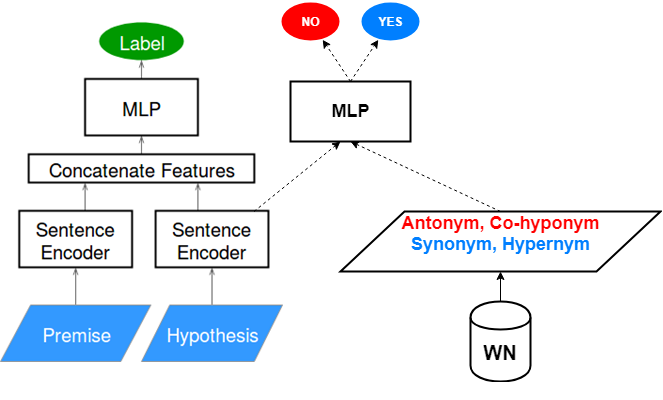
\includegraphics[totalheight=5.5cm]{fig/mt_architecture.png}
	\caption{Architecture of the Residual-Stacked Encoder with multitask learning for the sentence-representations.}
	\label{fig:mt_architecture}
\end{figure}
The left side shows the standard architecture of the Residual-Stacked Encoder, as defined in Section §\ref{sec:residual_encoder_def}. Both sentences $p$ and $h$ are encoded using the same sentence encoder. The resulting sentence-representations are concatenated with the additional features and classified by the final \ac{MLP} into on the three labels entailment, neutral or contradiction. The additonal \ac{MLP} on the right side is used for the helper task. We create the helper-task with the intention to force the model to encode differences between two words $w_1$ and $w_2$, if one is the antonym or co-hyponym of the other.  Likewise, if $w_1$ and $w_2$ are synonyms or $w_2$ is the hypernym of $w_1$ and thus entailed by it, we want this information to be encoded as well. We define our helper task as a binary classification problem, whether a word (or its meaning) is encoded (or entailed) within the sentence representation or not. For this, we consider both sentences $p$ and $h$ from a \ac{BoW} perspective. Let $S=\{w^0, w^1 , \ldots, w^{n-1}, w^n\}$ be the set of all $n$ distinct words $w$ within a sentence. We apply the same task for $p$ and $h$. Since we do not consider them simultaneously but individually, we define the helper-task using the general $S$ respectively for both. For each $w^i \in S$, we identify words from WordNet, being linked to $w^i$ with one of the previously mentioned relations. Let $A$ be the set of words, whos meaning must be entailed by the sentence representation, thus $A$ contains all hypernyms and synonyms of all $w^i \in S$. Similarily, let $B$ be the set of words, who's meaning is \textit{not} entailed by the sentence, thus antonyms and co-hyponyms of all $w^i \in S$. Additionally, all $w^i$ that have related words via lexical semantic relations are also added to $A$. A sentence like ``People are watching a soccer game between Brazil and Mexico.'' may still cause conflicts, as $A$ contains ``Brazil'' and ``Mexico'', however they may also be present within $B$, being mutual co-hyponyms. To avoid conflicts, if several co-hyponyms are present within the same sentence, we ensure that $A$ and $B$ are not overlapping, by setting $B = B \setminus (S \cup A)$. The final helper-task takes a sentence-representation $r$ and a word embedding $e$ as input, and must classify, whether $e$ belongs to $A$ or $B$, meaning whether $e$ is present (in the sense of entailment) within $r$ or not. Since the same embeddings are used and fine-tuned, this may also be seen as a postprocessing step for word vectors like in Attract-Repel \citep{vulic2017specialising}, but additionally ensuring, those differences are propagated into the sentence-representation. 

\paragraph*{Training}
The main-task and the helper-task are simultaneously trained. Thus, the combined loss, denoted as $loss_\text{combined}$, aggregates the loss for the main-task, denoted as $loss_\text{main}$, and for the helper task, denoted as $loss_\text{helper}$:
\begin{equation}
\label{eq:multitask_aggregate}
\text{loss}_\text{combined} = \alpha \text{ loss}_\text{main} + (1 - \alpha)\text{ loss}_\text{helper}
\end{equation}
Here, $\alpha \in \{x \in \mathbb{R} | 0 \leq x \leq 1\}$ regulates the impact of the main-task, with a high value ($\alpha = 1$) only considering the main-task and a low value ($\alpha = 0$) only the helper-task. While $loss_\text{main}$ remains the original mean cross-entropy, $loss_\text{helper}$ is also based on mean cross-entropy, yet is down-weighted for the following reason. Let $A_p$, $B_p$ and $A_h$, $B_h$ be $A$ and $B$ according to the definitions above for $p$ and $h$ respectively and $|A|$ denote the amount of samples within a set $A$. One can safely assume, that the amount of samples for the helper-task is tremendously higher than for the main task, since one single sample ($p$,$h$) in this task yields $|A_p|+|B_p|+|A_h|+|B_h| \gg 1$ samples in the helper-task. Let $b$ be the batch-size and $p^i$ and $h^i$ denote the $i$th $p$ or $h$ within a minibatch. We calculate $n$ to be the total amount of samples for the helper-task within a given batch:
\begin{equation}
n = \sum^b_{i=1}\Big(|A_{p^i}|+|B_{p^i}|+|A_{h^i}|+|B_{h^i}|\Big)
\end{equation}
Let $loss_\text{s}$ be the loss, calculated with mean cross-entropy, for all samples coming from $A_s$, $B_s$, with $s$ being any sentence $p$ or $h$. The re-weighted $loss_\text{helper}$ over all ($p$, $h$) within a minibatch is calculated as:
\begin{equation}
\text{loss}_\text{helper} = \sum^b_{i=1}\bigg( \frac{|A_{p^i}| + |B_{p^i}|}{n} \text{loss}_{\text{p}^i} + \frac{|A_{h^i}| + |B_{h^i}|}{n} \text{loss}_{\text{h}^i} \bigg)
\end{equation}

\paragraph*{Multitask variations}
We evaluate several implementations with small differences or changed hyperparameters, following the presented architecture. Those are described below, mostly differing in their impact on the sentence-representation. 
\begin{itemize}
\item \textbf{Size and amount of layers:} We evaluate different sizes of the helper-task \ac{MLP}. Naturally, the simpler the helper-network (fewer layers or dimensions), the more information must be encoded within the representation. This should be preferrable, since finally we aim for the main-task to leverage from the same, hopefully meaningful, features, and we do not have further use of the \ac{MLP} of the helper-task.
\item  \textbf{Dropout:} Similarily, by using dropout (0.1) in the helper-task, we motivate the creation of redundant features within the sentence-representation.
\item \textbf{Re-sample less frequent label:} We observe that usually $|A_s| < |B_s|$, resulting especially from the large amount of co-hyponyms. In order to prevent the helper task to take the label distribution into account rather than creating relevant features, we re-sample the less frequent class of $A_s$ or $B_s$, such that $|A_s| = |B_s|$.
\item \textbf{Reweighting tasks:} By either statically adapting the value of $\alpha$ beforehand, or dynamically updating it during training, we change the impact of each task. Specifically, in the \textit{finetune}\footnote{$\alpha$ for 10 iterations: $\alpha = [0.5, 0.5, 0.5, 0.5, 0.5, 0.75, 1.0, 1.0, 1.0, 1.0]$} setting, at first both tasks have an equal impact, while in the end only the main task is considered. In the setting \textit{focus-start}\footnote{$\alpha$ for 10 iterations: $\alpha = [0.0, 0.5, 0.5, 0.5, 0.5, 0.5, 0.5, 0.5, 0.5, 1.0]$}, the encoder first creates a useful representation for the helper task only and afterwards also considers the main task. As opposed to that, in \textit{focus-mid}\footnote{$\alpha$ for 10 iterations: $\alpha = [1.0, 1.0, 1.0, 0.5, 0.0, 0.25, 0.5, 1.0, 1.0, 1.0]$}, we first tune the sentence-representation only for \ac{SNLI}, adapt this representation then for the helper task and finally finetune to \ac{SNLI} again.
\item \textbf{Freeze helper-task weights:} To not encode too much logic in the helper \ac{MLP}, we freeze the weights after one iteration, dentoted as \textit{(freeze)}. Subsequent enhancements must afterwards be encoded directly in the sentence representation. 
\item \textbf{Additional weight matrix on top of sentence-encoder:} In order to achieve a strong accuracy for the helper task, more than one layer is required in the \ac{MLP}. We use a two layer \ac{MLP} for the helper task. The main task however, does not depend on the original sentence-representation anymore, but on the output of the first layer of the helper-task \ac{MLP}. We name this configuration \textit{(shared)} in the evaluation.
\item \textbf{Focus on responsible words:} Instead of using all values, encoded within the sentence-representation, we follow the same approach as described in Section §\ref{sec:understanding}, identifying which word is responsible for which dimension, and focus the network on those explicit dimensions. Thus, we consider the original pairs ($w_1$, $w_2$, \texttt{relation}) and set all dimensions within the sentence-representation to zero, if they do not arise from $w_1$. Subsequent steps remain unchanged. This is motivated by the high amount of noise from the extracted WordNet data, especially for samples within $B$. Hence, the helper-task, that should focus on the relation between $w_1$ and $w_2$, may not depend on dimensions of $w_1$, but on arbitrary other dimensions. In this particular case we do leave $B$ untouched (and do not calculate it as $B  = B \setminus (S \cup A)$), since the conflict is resolved by focusing on different parts of the sentence-representation. We refer to \textit{(max-pool)}, when applying this strategy.
\end{itemize}
\subsection{Extraction of WordNet data}
We experiment with different strategies, how to extract relevant data from WordNet, considering the lexical semantic relations, as described in Section §\ref{sec:word_relations}. We find, that by aiming for a high recall (thus considering \textit{all} senses of each word), a lot of noise is added, especially for co-hyponyms. For instance consider the word ``blue'', which is almost always used as a color. Yet, ``blue'' contains 16 different senses in total, ranging from ``sky'', ``amobarbital sodium'' or a ``family of butterflies'' to adjectives like ``aristrocratic'' or ``depressed''. This yields in antonyms like  ``lowborn'', ``cheerful'' or ``clean''. The impact is even stronger, when identifying co-hyponyms. As seen in Section §\ref{sec:wordnet}, WordNet maintains in many, but not in all cases, a very fine-grained hypernomy graph, requiring us to not only consider the next hypernym, but several hypernyms along the path. Doing so, words like ``miller'' (a type of a moth) are considered as co-hyponym, naturally in an increasing frequency, as co-hyponyms in a tree-like structure appear exorbitantly more often than antonyms or synonyms.

\subsubsection{Strategy to extract data}\label{sec:used_wordnet_extract_strategy}
Instead of the previously explained approach, we only consider the first synset to detect related synsets via the lexical relations. This does not remove noise, yet reduces it. This comes with the cost of neglecting many useful lexical semantic relations, or even using the majorily wrong sense\footnote{In Section §\ref{sec:wordnet} we showed that table (in the sense of a tabular visualization) is the first sense of table (as opposed to the sense of a furniture). Yet, in \ac{SNLI} we especially expect the second sense to be useful.}. The main motivation is, that we lack of automatic evaluation methods for the extracted data w.r.t. \ac{SNLI}, conflicting with the time constraints for the remainder of the work. Since previous experiments\footnote{Conducted by Vered Shwartz and not part of this work.} focused on a high recall and did not improve the performance, we now aim for a high precision of the extracted data. Note, that the WordNet baseline, as defined in Section §\ref{sec:additional_snli_set} did not suffer from the same problem, since all word-pairs ($w_p$, $w_h$) already are known to have a meaningful relation (based on their creation process), thus the extracted relation between both words most likely is valid. The problem only occurs, as we intend to extract words the other way around, by knowing the relation.

\subsubsection{Final extracted data}
We consider all lemmata within the first synset of $w$ as synonyms. Hypernyms of $w$ are considered up to an edge length of 5. For co-hyponyms, we consider all hyponyms of hypernyms of $w$, both bound to an edge length of three, only if they are not also a hypernym of $w$. 
\begin{table}[tph!]
\centering
\begin{tabular}{cc|cc}
\multicolumn{2}{c}{\textbf{$\mathbf{A}$ (entailed)}} & \multicolumn{2}{c}{\textbf{$\mathbf{B}$ (contradicting)}} \\
\textbf{$\mathbf{w_1}$} & \textbf{$\mathbf{w_2}$} & \textbf{$\mathbf{w_1}$} & \textbf{$\mathbf{w_2}$} \\
\toprule
oppose & content & Trojan & Iraqi\\
pug & dog & waffle & Cheesecake\\
reward & rewarding & five & trio \\
townspeople & town & inferno & radius \\
pop & bulge & conditioner & aerobics\\
permit & permit & killers & party\\
frolics & play & hiding & processes\\
leading & ahead & chapel & synagogue\\
commitment & sincerity & Villages & crossroads\\
Wool & material & saloon & Minivan\\
\bottomrule
\end{tabular}
\caption{Examples of extracted word-pairs ($w_1$,$w_2$) for both categories, being represented by the sentence containing $w_1$ ( thus $A$) or not (thus $B$).}
\label{tab:examples_extracted_wn}
\end{table}
We also consider \textit{part-meronyms}, that are a hyponym of ``location'' of any distance. Since the interpretation of meronyms is not trivial w.r.t. entailment, we thus only consider it in the context of locations and assume that a meronym entails its holonym\footnote{As in ``John is in Berlin.'' $\Rightarrow$ ``John is in Germany.'', with ``Berlin'' \textit{part-of} ``Germany''}. We generate a total of 686,265 word pairs with their entailment interpretation into either $A$ or $B$, precisely $|A|=104,550$ and $|B|=581,715$. Note that these include the word itself like ($w_1$,$w_1$, $A$), if lexical semantic relations for a $w^s$ are found. All words appear within the \ac{SNLI} dataset and thus can be useful. We show random samples of ten pairs for each class respectively in Table \ref{tab:examples_extracted_wn}.
Obviously, the data is still not entirely clean, however one can at least identify, why several word-pairs are within $A$ or $B$. Applying the extracted data on sentences within \ac{SNLI} train data, yields to an average of 44.6 samples from $A$ and 300.0 samples from $B$ for the helper-task for each single sentence, $p$ or $h$.
\subsection{Evaluation}
We evaluate all previously explained experiments within this section.
\subsubsection{Integrate WordNet using embeddings}
Table \ref{tab:eval_embeddings_added} shows the performance of the concatenated word-embeddings together with the performance of the unchanged Residual-Stacked Encoder\textsuperscript{$\dagger$}. The upper part contains embeddings that have been newly created or changed to contain other than (only) distributional information, the lower part shows the concatenated hypernyms, using the original (but fine-tuned during training) distributional representations.
\begin{table}[tph!]
\centering
\begin{tabular}{rc|cc|cc}
\textbf{Additional Embeddings} &\textbf{Dimensions} & \textbf{\ac{SNLI} test} & \textbf{$\Delta$} & \textbf{New test} & \textbf{$\Delta$}\\
\toprule
Attract-Repel \citep{ruckle2018concatenated} & 300D & 85.4\% & $-$0.4 & 58.3\% & $-$0.9 \\
Trained-All (cross-entropy) & 50D & 85.4\% & $-$0.4 & 59.2\% & $\pm$0 \\
Trained-Syn-Ant (eucledian) & 20D & 85.4\% & $-$0.4 &57.8\% & $-$1.4 \\
Trained-Syn-Cohyp (eucledian)& 20D & 85.5\% & $-$0.3 &55.7\% & $-$3.5 \\
Trained-Syn-Cohyp-Ant (eucledian)& 20D+20D & 85.7\% & $-$0.1 & 56.6\% &  $-$2.6 \\
\midrule
Hypernyms-1 & 300D  & 85.2\% & $-$0.6 & 54.8\% & $-$4.4 \\
Hypernyms-3 & 300D  & 85.3\% & $-$0.5 & 60.8\% & $+$1.6 \\
Hypernyms-5 & 300D  & 85.4\% & $-$0.4 & 66.4\% & $+$7.2 \\
\midrule
\textbf{Residual-Stacked Encoder\textsuperscript{$\dagger$}} & $-$ & 85.8\% &$\pm$0 & 59.2\% & $\pm$0\\
\bottomrule
\end{tabular}
\caption{Evaluation of experiments with additional information in the word-representations, compared to the Residual-Stacked Encoder\textsuperscript{$\dagger$} (bottom).}
\label{tab:eval_embeddings_added}
\end{table}
All methods slightly decrease in terms of accuracy for the original \ac{SNLI} test set, even though only additional information is added. This however is not significant and most likely stems the parameters being highly tuned towards \ac{SNLI} for the original model. Since we do not intend to increase the performance by a small margin coming from hyperparameter settings, we do not fine-tune these. Also on the new test set, most approaches do not show major differences to the original model. Only the concatenation of hypernyms shows with an increasing amount improvements, which is even stronger than the accuracy achieved by \ac{ESIM} \citep{chen2017enhanced}. 
\subsubsection{Integrate WordNet using multitask-learning}\label{sec:eval_mt}
We depict the results of experiments using multitask-learning, as described in Section \ref{sec:mt_learning_intro}, in Table \ref{tab:mt_evaluation}.
\begin{table}[tph!]
\centering
\resizebox{\textwidth}{!}{%
\begin{tabular}{rccc|cr|cr}
\textbf{Helper-task MLP} & $\alpha$ & \textbf{dropout} & \specialcellc{\textbf{Re-sample}\\\textbf{less frequent}} & \textbf{\ac{SNLI} test} & $\Delta$ & \textbf{New test} & $\Delta$ \\
\toprule
2 $\times$ 100D & 0.5 & $-$ & yes & 84.6\% & $-$1.2 & 47.2\% & $-$12.0 \\
2 $\times$ 600D & 0.5 & $-$ & yes & 85.2\% & $-$0.6 & 59.9\% & $+$0.7 \\
2 $\times$ 300D & 0.5 & yes & yes & 84.8\% & $-$1.0 & 52.5\% & $-$6.7 \\
2 $\times$ 600D & 0.5 & yes & yes & 84.8\% & $-$1.0 & 51.8\% & $-$7.4 \\
2 $\times$ 300D & 0.5 & yes & $-$ & 85.2\% & $-$0.6 & 48.7\% & $-$10.5 \\
2 $\times$ 600D & 0.5 & yes & $-$ & 85.0\% & $-$0.8 & 57.7\% & $-$1.5 \\
2 $\times$ 300D & 0.75 & yes & yes & 85.3\% & $-$0.5 & 61.0\% & $+$1.8 \\
2 $\times$ 300D & 0.75 & yes & $-$ & 85.7\% & $-$0.1 & 58.9\% & $-$0.3 \\
\midrule
2 $\times$ 300D & \texttt{finetune} & yes & yes & 84.9\% & $-$0.9 & 51.5\% & $-$7.7 \\
2 $\times$ 300D & \texttt{finetune} & $-$ & yes & 84.5\% & $-$1.3 & 52.3\% & $-$6.9 \\
2 $\times$ 600D & \texttt{focus-start} & $-$ & yes & 85.4\% & $-$0.4 & 46.9\% & $-$12.3 \\
2 $\times$ 600D & \texttt{focus-mid} & $-$ & yes & 85.4\% & $-$0.4 & 59.6\% & $+$0.4 \\
\midrule
2 $\times$ 300D (freeze) & 0.75 & $-$ & yes & 85.3\% & $-$0.5 & 53.2\% & $-$6.0 \\
2 $\times$ 300D (freeze) & 0.5 & $-$ & yes & 84.7\% & $-$1.1 & 44.8\% & $-$14.4 \\
2 $\times$ 800D (shared) & 0.5 & yes & yes & 84.4\% & $-$1.4 & 42.2\% & $-$17.0 \\
2 $\times$ 600D (shared) & 0.75 & yes & yes & 84.6\% & $-$1.2 & 42.3\% & $-$16.9 \\
2 $\times$ 400D (shared) & 0.5 & yes & yes & 83.9\% & $-$1.9 & 34.3\% & $-$24.9 \\
\midrule
2 $\times$ 300D (max-pool) & 0.75 & yes & yes & 84.8\% & $-$1.0 & 57.8\% & $-$1.4 \\
\midrule
\textbf{Residual-Stacked Encoder\textsuperscript{$\dagger$}} &$-$&$-$&$-$&85.8\%&$\pm$0&59.2\%& $\pm$0 \\
\bottomrule

\end{tabular}}
\caption{Evaluation of experiments using multitask-learning, compared with the Residual-Stacked Encoder\textsuperscript{$\dagger$.}}
\label{tab:mt_evaluation}
\end{table}
The first column shows the dimensions of the helper-task \ac{MLP}. We only used two layer \ac{MLP}s with the specified dimensions, as previous experiments showed that smaller networks have already problems reaching a high accuracy of the helper-task. The presented networks all solve this task with an accuracy of $> 90 \%$ (dev). Similarily, we observe that, reducing  $\alpha$, thus increasing the impact of the helper-task, in most cases reduces the performance on the main task. Generally, reducing the impact of the helper-task, by increasing the complexity of the helper-task \ac{MLP}, omitting dropout or by increasing $\alpha$, the performance drops less (or slightly improves). Subsequently, experiments with a very strong impact of the helper task, as sharing a layer of its \ac{MLP} or freezing its weights, result in a very poor performance. The dynamic adaptions of $\alpha$ in the second part of the table only show comparable results to the original model, if the helper-task is considered for a few iterations only. By taking max-pooling information into account, the performance decreases slightly. While this potentially should lay the focus on relevant words, we neglect the fact, that certain attributes may be shifted, due to the context implementing nature of \ac{LSTM}s. Thus, for ``a happy child'' the information for \textit{being happy} might not only be present within ``happy'', but also within ``child'', as the first describes the second word. This may result in ``child'' having a higher value within the relevant dimension. While this dimension for ``happy'' may still be relatively high, in our experiment we would neglect this dimension completely (by setting it to zero), when predicting ``happy'' in the helper-task. Thus a more sophisticated approach might be, to consider the output vectors after each timestep for the according word directly, instead of masking the final sentence representation. Re-sampling the helper task such that $|A| = |B|$ seems superior to not-resampling.

\subsection{Analysis}
We analyse selected experiments of both approaches in this section.

\subsubsection{Integrate WordNet using embeddings}
\begin{table}[tph!]
\centering
\begin{tabular}{rcc|cr|cr}
\textbf{Category}  & \textbf{Amount}& \specialcellc{\textbf{Residual-Stacked}\\\textbf{Encoder}\textsuperscript{$\dagger$}} & \specialcellc{\textbf{Attract-}\\\textbf{Repel}} & $\Delta$ &  \textbf{Hypernyms-5} & $\Delta$ \\
\toprule
antonyms & 1,147 & 51.0\% & 53.8\% & $+$2.8 & 74.2\% & $+$23.2 \\
cardinals & 759 & 20.3\% & 19.1\% & $-$1.2 & 15.3\% & $-$5.0 \\
nationalities & 755 & 44.2\% & 31.1\% & $-$13.1 & 56.7\% & $+$12.5 \\
drinks & 731 & 89.7\% & 93.3\% & $+$3.6 & 72.7\% & $-$17.0 \\
antonyms(WN) & 706 & 63.2\% & 60.8\% & $-$2.4 & 71.2\% & $+$8.0 \\
colors & 699 & 90.8\% & 88.1\% & $-$2.7 & 95.2\% & $+$7.1 \\
ordinals & 663 & 3.0\% & 8.8\% & $+$5.8 & 6.2\% & $+$3.2 \\
countries & 613 & 75.4\% & 44.1\% & $-$31.3 & 81.6\% & $+$6.2 \\
rooms & 595 & 73.1\% & 77.0\% & $+$3.9 & 75.0\% & $+$1.9\\
materials & 397 & 80.4\% & 77.6\% & $-$2.8 & 85.1\% & $+$4.7 \\
vegetables & 109 & 40.4\% & 41.3\% & $+$0.9 & 41.3\% & $+$0.9 \\
instruments & 65 & 96.9\% & 98.5\% & $+$1.6 & 98.5\% & $+$1.6 \\
planets & 60 & 61.7\% & 31.7\% & $-$30.0 & 38.3\% & $-$23.4 \\
\midrule
synonyms & 894 & 73.9\% & 92.6\% & $+$18.7 & 74.9\% & $+$1.0 \\
\midrule
total & 8,193 & 59.2\% & 58.3\% & $-$0.9 & 66.4\% & $+$7.2 \\
\bottomrule
\end{tabular}
\caption{Accuracy per category for concatenated embeddings using Attract-Repel or Hyponyms-5.}
\label{tab:detail_added_embds}
\end{table}
Table \ref{tab:detail_added_embds} shows the accuracy per category for \textit{Attract-Repel}, as being the most sophisticated word-representations with additional non-distributional information and \textit{Hypernyms-5}, as the best achieved result. Comparing the model using concatenated embeddings from Attract-Repel with the Residual-Stacked Encoder\textsuperscript{$\dagger$} indicates, that different features are considered relevant by the netwrok. Most of the differences within the categories seem arbitrary, arising most likely from this different feature selection, as the original information would still be accessable to the model. Synonyms are strongly improved compared to the original model, which can easily be explained due to an even higher word-vector similarity from Attract-Repel post-processed representations. On the other hand, both antonym groups show no substantial improvement. The antonyms derived from WordNet show an even worse accuracy than before. Overall, the performance gained using these embeddings with all deviations within different categories is highly similar to the ones achieved using multitask learning (next Section). Since the added word-vectors encode differences for most antonyms, but do not leverage them, we assume this stems from a lack of representative data within \ac{SNLI} data. Naturally, if the model does not depend on those differences during training, it will not learn to consider them in the prediction process.

\paragraph*{Impact of hypernyms}
Looking at the concatenation with the hypernyms for each word, the increase in performance looks much more stable. Ignoring \textit{planets}, which are highly noise-sensitive due to their limited size, only two categories do not improve over the baseline. Synonyms also (like mutually exclusive words) share similar hypernyms, the model must learn this differentiation. Looking at the categorical evaluation, the performance of synonyms remains similar to the original evaluated model, the Residual-Stacked Encoder\textsuperscript{$\dagger$}, showing that it does not suffer from added hypernyms in this aspect. Yet, we observe that adding hypernyms does not help in identifying synonyms, which is based on the results in Section §\ref{sec:additional_snli_set} a relatively easy to classify category. Especially the overall improvement for contradicting examples is interesting and we closer examine the impact of the hypernyms for these samples. To focus on the actual impact of the new information, we exclude all samples that are predicted identically as by the Residual-Stacked Encoder\textsuperscript{$\dagger$}, thus exclude samples that are correctly classified based on memorizing word-relations. 
\begin{figure}[tph!]
\centering
	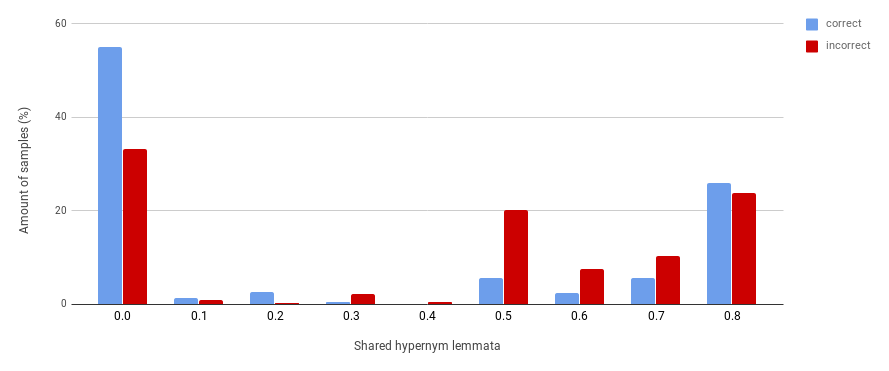
\includegraphics[totalheight=5.5cm]{fig/analyse_hypern5.png}
	\caption{Comparison of contradicting samples (different w.r.t. correctness from Residual-Stacked Encoder\textsuperscript{$\dagger$}). for Hypernyms-5, by the amount of shared hypernym embeddings.}
	\label{fig:analyse_hypern5}
\end{figure}
Figure \ref{fig:analyse_hypern5} visualizes the impact of the hypernym embeddings by comparing how many hypernym embeddings are shared for each word-pair($w_p$,$w_h$). In total, 1378 contradicting samples are classified differently from the original model, 984 are now classified correctly as contradiction (blue), 394 samples are now misclassified (red). The x-axis shows the percentage $x_{w_p,w_h}$ of shared hypernym lemmata between $w_p$ and $w_h$, calculated as 
\begin{equation}
x_{w_p,w_h} = \frac{|H_{w_p} \cap H_{w_h}|}{|H_{w_p} \cup H_{w_h}|}
\end{equation}
with $H_{w_p}$ and $H_{w_h}$ being the sets lemmata of hypernyms from $w_p$ and $w_h$ respectively, gathered using the same method as to create the embeddings. The y-axis displays the proportional amount of each group. Contrarily to our intention, the model does not seem to use the additional vectors to identify co-hyponyms. Instead, especially if only few hypernyms are identical (fewer indicators for co-hyponym), more samples are re-predicted correctly, whereas a higher similarity of the hypernyms leads to a higher amount of incorrect predictions. The fact that those ``unrelated'' words are an indicator for contradiction highly correlates with the data seen during training. Due to the creation process of \ac{SNLI} (in addition to to frequently changed words as identified by \cite{gururangan2018annotation}) many contradicting samples describe very unrelated scenarios, yielding in contradiction based on the event-coreference, not because they contain related, but contradicting, words \citep{dasgupta2018evaluating}. Subsequently, unrelatedness of words serves as a good indicator for contradiction. Yet, looking at categories individually, we observe that at least for some of them, the model learned the tendency of leveraging from the added information in the intended way. Correct classified cardinals in general all share $\geq 0.7$ \% of their hypernym lemmata, thus are very similar to each other. A total of 200 cardinal samples are either in the red or blue group visualized. Of those, 143 (71.5\%) have been classified correctly with the concatenated hypernyms and only 57 (28.5\%) are misclassified compared to the original predictions. Similar, but less strongly, are 63 (61.8\%) countries with $\geq 0.7$\% shared hypernym lemmata classified correctly, and only 39 (38.2\%) incorrectly. Opposed to these categories, for nationalities or antonyms, the improvements compared to the base model arises from unrelated word-pairs (in terms of their shared hypernym lemmata). In both cases, the majority of different re-prediction stems from word-pairs sharing no lemma within their hypernyms. Only looking at those word-pairs, sharing not a single word-vector for their hypernyms, 109 (88.6\%) of 123 nationalities\footnote{Other \textbf{mispredictions}: 2$\times$ with 0.8 shared, 3$\times$ with 0.3 shared. Other \textbf{correct} predictions: 5$\times$ with 0.1$-$0.5 shared, 16$\times$ with 0.7$-$0.9 shared} and 278 (90.3\%) of 308 antonyms\footnote{Other \textbf{mispredictions}: 52 $\times$ 0.5$-$0.9 shared. Other \textbf{correct} predictions: 5$\times$ with 0.2$-$0.5 shared, 41 with 0.5$-$0.9 shared.} are re-predicted correctly. In total, the model seems to slightly benefit from the added information in some cases in the intended way, in the majority of cases however, the improvement in performance seems to stem from another frequently occuring pattern in \ac{SNLI}, namely unrelated hypotheses, rather than improving the general \ac{NLU}. 

\subsubsection{Integrate WordNet using multitask-learning}
For the analysis of multitask-learning we select the best performing model on the new test-set using a 300-dimensional helper task \ac{MLP} with $\alpha=0.75$ with re-sampling and dropout, denoted as \textit{300D-0.75 STD} and the comparable model with with a stronger impact of the helper-task with $\alpha=0.5$, also 300 dimensions, re-sampling and dropout, named as \textit{300D-0.5 STD}. Additionally, we select the model using the max-pooled information, referred to as \textit{300D-0.75 max-pool}, as it puts the focus on the actual word relations and performs comparably with the Residual-Stacked Encoder\textsuperscript{$\dagger$}. The accuracy per category of these models is displayed in Table \ref{tab:categories_mt}.
\begin{table}[tph!]
\centering
\begin{tabular}{rc|cr|cr|cr}
\textbf{Category}  & \textbf{Amount}& \specialcellc{\textbf{300D-0.75}\\\textbf{STD}} & $\Delta$ &  \specialcellc{\textbf{300D-0.5}\\\textbf{STD}} & $\Delta$ & \specialcellc{\textbf{300D-0.75}\\\textbf{max-pool}} & $\Delta$\\
\toprule
antonyms & 1,147 & 39.4\% & $-$11.6 & 35.6\% & $-$15.5 & 44.9\% & $-$6.1 \\
cardinals & 759 & 40.1\% & $+$19.8 & 26.2\% & $+$5.9  & 33.3\% & $+$13.0\\
nationalities & 755 & 52.5\% & $+$8.3 & 32.1\% & $-$12.1 & 25.3\%  & $-$18.9\\
drinks & 731 & 75.9\% & $-$13.8 & 67.4\% & $-$22.3 & 82.5\% & $-$7.2\\
antonyms(WN) & 706 & 60.5\% & $-$2.7 & 56.2\% & $-$7.0 & 56.5\% & $-$6.7\\
colors & 699 & 90.6\% & $-$0.2 & 86.3\% & $-$4.6 & 88.0\% & $-$2.8\\
ordinals & 663 & 3.0\% & $\pm$0 & 2.7\% & $-$0.3 & 3.2\% & $+$0.2\\
countries & 613 & 69.8\% & $-$5.6 & 40.6\% & $-$34.8 & 69.7\% & $-$5.7\\
rooms & 595 & 74.1\% & $+$1.0 & 65.2\% & $-$7.9 & 74.6\% & $+$1.5\\
materials & 397 & 85.9\% & $+$5.5 & 79.8\% & $-$0.6 & 72.3\% & $-$8.1\\
vegetables & 109 & 41.3\% & $+$0.9 & 44.0\% & $+$3.6 & 32.1\% & $-$8.3\\
instruments & 65 & 95.4\% & $-$1.2 & 93.8\% & $-$3.1 & 95.4\% & $-$1.5\\
planets & 60 & 35.0\% & $-$26.7 & 26.7\% & $-$35.0 & 58.3\% & $-$3.4\\
\midrule
synonyms & 894 & 97.6\% & $+$23.7 & 96.1\% & $+$22.2 & 94.4\% & $+$19.5\\
\midrule
total & 8,193 & 61.0\% & $+$1.8 & 52.5\% & $-$6.7 & 57.8\% & $-$1.4\\
\bottomrule
\end{tabular}
\caption{Accuracy per category for selected models using multitask-learning.}
\label{tab:categories_mt}
\end{table}
It can be seen that the majority of all contradicting categories performs worse than the base-model. Only the synonyms highly leverage from this method and reassemble the performance reached by attention-based models in Section §\ref{sec:additional_snli_set}. We observe this phenomenon on synonyms for all 17 evaluated models of Section §\ref{sec:eval_mt}. The extracted synonyms from WordNet are much less noisy than co-hyponyms, indicating that the helper-task is more likely to consider the relevant dimensions coming from the synonym for its prediction. However, as seen by the model taking max-pooling information into account, the performance on contradicting samples is still very poor. Only two categories seem to be improved on a relatively constant basis. Cardinals improve in 7/17 approaches, mostly by more 10 ten points in accuracy, vegetables improve in 9/17 approaches, with a maximum of 9.1\% increase. Especially the drop within the second model for countries is severe, yet not only present within this experiment. Not a single model of our evaluations superceeded the original model for countries, 8/16 decreased by more than 35 points in accuracy, another 2 experiments by more than 10 points. Since the other models of Section §\ref{sec:additional_snli_set} achieve similar results, and Residual-Stacked Encoder\textsuperscript{$\dagger$} is highly aligned with its hyperparameters to Residual-Stacked Encoder\textsuperscript{$\Diamond$}, we assume the high performance arises from correctly picked features by chance, rather than stemming from the model's architecture. 

\paragraph*{Impact of the selected data}
Due to the restricted method of extracting word-pairs, defined in Section §\ref{sec:used_wordnet_extract_strategy}, the upper bound, that can be achieved using this information drops. Thus, in the following analysis we only look at samples, that could have been classified correctly, based on this extracted data from WordNet. The results are depicted in Table \ref{tab:eval_mt_data}. We report the absolute amount of samples together with the percentage, compared to the original size of each category. The categories drinks (3), instruments (11), vegetables (20), materials (35) and planets (37) are aggregated, due to insufficient amount of samples for any representative conclusions. All $\Delta$ show the difference to the Residual-Stacked Encoder\textsuperscript{$\dagger$} on the same data, instead of comparing them with the same model using the full data.
\begin{table}[tph!]
\centering
\resizebox{\textwidth}{!}{%
\begin{tabular}{rccc|cr|cr|cr}
&\multicolumn{2}{c}{\textbf{Amount}}& \specialcellc{\textbf{Residual-Stacked}\\\textbf{Encoder\textsuperscript{$\dagger$}}} & \multicolumn{2}{c}{\textbf{300D-0.75 STD}} & \multicolumn{2}{c}{\textbf{300D-0.5 STD}} & \multicolumn{2}{c}{\specialcellc{\textbf{300D-0.75}\\\textbf{max-pool}}}\\
\textbf{Category} & \# & \% & Acc. & Acc.& $\Delta$ & Acc.& $\Delta$ & Acc.& $\Delta$\\
\toprule
antonyms & 885 & 77.2\% &51.3\% &37.7\%&$-$13.6&36.5\% &$-$14.8  &46.6\% &$-$4.7\\
cardinals &496 &65.3\%&21.6\% &41.2\%&$+$19.6&29.6\% &$+$8.0 &34.7\% &$+$13.1\\
countries & 471&76.8\% &75.6\% &66.2\%&$-$9.4&33.3\% &$-$42.3 &68.2\% &$-$7.4\\
nationalities &427 & 56.6\% &43.4\% &59.3\%&$+$15.9&32.8\% &$-$10.6 &32.1\% &$-$11.3\\
antonyms(WN) &379 & 53.7\%&77.6\% &76.0\%&$-$1.6&70.8\% &$-$6.8 &69.7\% &$-$7.9\\
colors & 312& 44.6\%&95.8\% &95.8\%&$\pm$0&93.3\% &$-$2.5 &93.3\% &$-$2.5\\
ordinals &263 &39.7\% &6.5\% &7.2\%&$+$0.7&6.5\% &$\pm$0 &6.5\% &$\pm$0\\
rooms &213 &35.8\% &94.8\% &85.4\%&$-$9.4&76.1\% &$-$18.7 &95.3\% &$+$0.5\\
\textit{other} & 106 & 7.8\% & 33.0\% &48.0\%&$+$15.0&52.8\% &$+$19.8 &33.0\% &$\pm$0\\
\midrule
synonyms & 385& 43.1\% &98.2\% &100.0\%&$+$1.8&99.7\%&$+$1.5  & 100\%& $+$1.8\\
\midrule
\textbf{Total} & 3,937 & 48.1\% & 60.1\%&59.5\%&$-$0.6&49.7\% &$-$10.4 &57.5\% &$-$2.6 \\
\bottomrule
\end{tabular}}
\caption{Accuracy per category of three selected multitask-learning experiments compared with Residual-Stacked Encoder\textsuperscript{$\dagger$} on samples covered by extracted word-pairs.}
\label{tab:eval_mt_data}
\end{table}
The 100\% accuracy on synonyms is not very surprising, given the fact that only synonym examples are included, if they can be explained using the extracted data. Thus, samples of this category that have another label than entailment, due to the usage in context, are excluded. The performance gain in the aggregated \textit{other} category mostly stems from materials. All of the multitask experiments, generally perform worse than the base model without multitask-learning. If we compare the overall performance of each model on this subset of data with the performance achieved over all data, we observe that only the original Residual-Stacked Encoder\textsuperscript{$\dagger$} improved in accuracy, while other models perform worse than before. Subsequently, they perform slightly better on the other half of the data, that cannot be explained using the fused information. \cite{chen2017natural} show with \ac{KIM} and a total of 5,425,426 extracted word pairs\footnote{Note, that they align words of $p$ and $h$ to identify their relation, thus they may not suffer that much from arbitrary word relations, extracted from WordNet.}, being crucially more than ours, that the network especially leverages, if $\geq$ 40\% of the external knowledge is used. Compared too that, our experiments may indeed suffer from limited coverage, especially since \cite{chen2017natural} directly encode the lexical relations and we still rely on the \ac{MLP} to identify them, indirectly encoded within the sentence-representation. Yet, it could have been expected, that models would have an advantage on this subset of data either way. Since they obviously fail leverage from the fused information, sufficient for all those samples, the problem seems to rather be the method than the data.

\paragraph*{Impact on the sentence representation}
Looking back to the original intention, of fine-tuning embeddings and ensuring those differences would be present within the sentence-representation, we take a closer look at this aspect. Following the results from the previous step we can only see, that the multitask-learning is not heelpful for the final prediction, which can have several reasons: Either the helper-task did not manage to encode the relevant differences into the sentence-representation, or it did, but the model failed to use them. We use the same technique as introduced in Section §\ref{sec:approach_general_alignment_understanding}, visualizing the alignment of the sentence-representations of $p$ and $h$. We only calculate the averaged counts per dimension for the same subset of the data from the previous section, but only looking at contradicting samples (3511 in total).
\begin{figure}[tph!]
\centering
	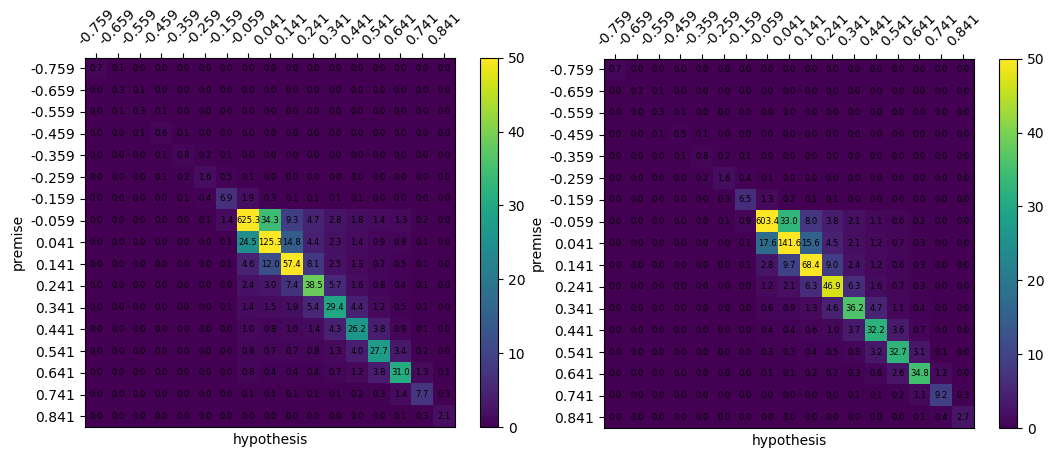
\includegraphics[totalheight=7cm]{fig/base_correct_incorrect_c.png}
	\caption{Aligned $p$ and $h$ for all contradicting sampes, covered by the fused WordNet information, correctly predicted (left) or mis-predicted (right).}
	\label{fig:base_correct_incorrect_c}
\end{figure}
Figure \ref{fig:base_correct_incorrect_c} shows the aligned sentences for the Residual-Stacked Encoder\textsuperscript{$\dagger$}, differentiating between the 1954 correctly classified samples and 1557 misclassified samples. As expected, the majority of dimensions have the same value, arising from the high lexical overlap and the fact that word-pairs are selected to be replacable in context, thus will have similar embeddings. Even though the network structure, dimensions and performance, compared to the analysed model Shortcut-Stacked Encoder\textsuperscript{$\dagger$}, slightly changed, the results gained from this section still seem applicable. Due to the similarity of both sentences, only few dimensions differ. We observe more of these differing high dimensions for the correctly classified samples, in many cases more than twice the amount compared to the misclassified samples. Knowing that the Residual-Stacked Encoder\textsuperscript{$\dagger$} most likely follows the same principles as identified in Section §\ref{sec:understanding}, we now look at the sentence-representations gained from multitask-learning (for the same data). Figure \ref{fig:300d75_correct_incorrect_c} shows the aligned sentence-representations (correct and misclassified) for the best multitask-learned model \textit{300D-0.75 ST}.
\begin{figure}[tph!]
\centering
	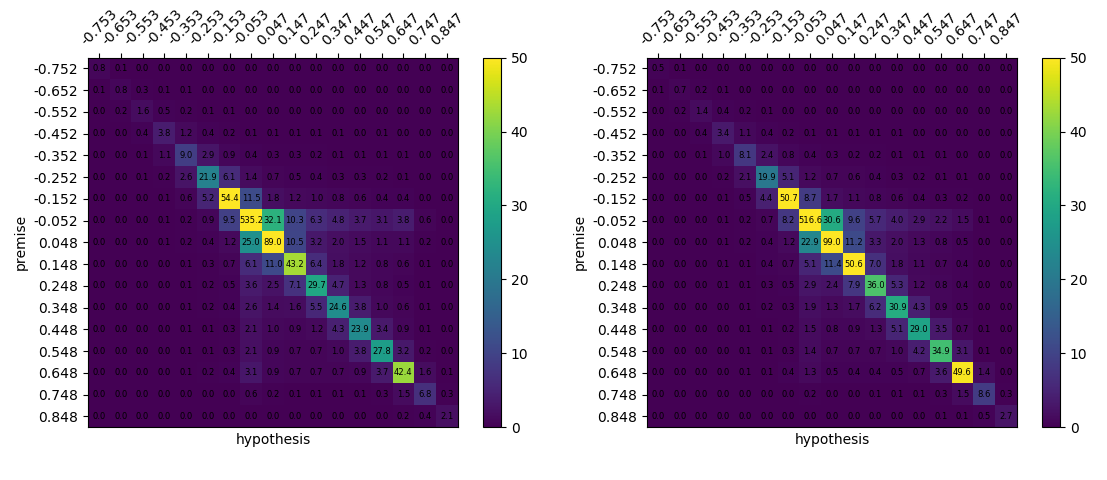
\includegraphics[totalheight=7cm]{fig/300d75_correct_incorrect_c.png}
	\caption{Aligned $p$ and $h$, correctly predicted (left) and mis-predicted (right) for multitask-learned \textit{300D-0.75 STD}.}
	\label{fig:300d75_correct_incorrect_c}
\end{figure}
Comparing these visualizations with the orignal model, clearly both, the mispredicted and correctly predicted sentence-representations show a higher amount of different high-valued dimensions. In line with our other observations, this is especially visible for the correctly classified samples. While the Residual-Stacked Encoder\textsuperscript{$\dagger$}, as well as the Shortcut-Stacked Encoder\textsuperscript{$\dagger$} showed the majority of dimensions within the positive values area, in this case a huge amount of samples are also within the negative area. We do not start another dimension-wise analysis for this model and leave it open for interpretation. Since this phenomenon stems from the helper-task, one possible explanation is, that low values indicate the absence of specific words. Having a large lexical overlap, $p$ and $h$ lack the identical words or meaning (coming from $B$) for the majority of words. Thus the dominant symmetry for the negative values may arise. Even though the main-task may still optimize to deal with negative values or interpret the absence of information within a dimension not aligned with zero but another value (as opposed to the original model), this breaks the same behaviour that was naturally learned by both models without multitask-learning. Similarily, \cite{mou2015natural} showed, that even though the model is able to learn element-wise difference and product (which both work intuitively well with absence of information being encoded close to zero) by themselves, using it in the feature concatenation helps the performance. Yet, we do not further investiate this phenomenon and it may not even be harmful to the final prediction. Similar results are shown for the other two experiments, picked for the analysis part\footnote{We did not conduct similar analysis for the remaining models.}. Figure \ref{fig:masking_e_c} shows all contradicting and entailing samples of the selected data, regardless of the prediction of the model, encoded by \textit{300D-0.75 max-pool}.
\begin{figure}[tph!]
\centering
	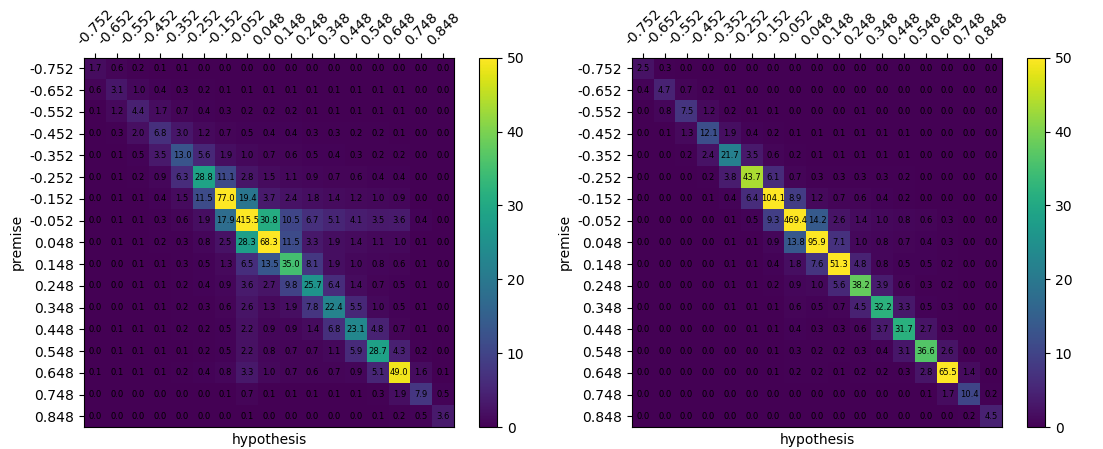
\includegraphics[totalheight=7cm]{fig/masking_e_c.png}
	\caption{Aligned $p$ and $h$, of contradicting (left) and entailing (right) samples for multitask-learned \textit{300D-0.75 max-pool}.}
	\label{fig:masking_e_c}
\end{figure}
This seems to be a bit more fuzzy, compared to the other two multi-tasking experiments. Neglecting the high amount of negative valued dimensions, this is exactly the kind of representations we were aiming for, clearly encoding the same information for entailing examples, while also encoding differences for the contradicting samples\footnote{This also can be seen for the other two evaluated models.}. As seen in Section §\ref{sec:understanding_align_neutral_contr}, this however is not sufficient for the model to predict contradiction, as distinct information is also present for neutral samples. We conclude, that we managed to shift the sentence-representation in a way, that it encodes differences for antonyms and co-hyponyms stronger than before. However the classifying \ac{MLP} lacks to leverage from those in the intended way. 
\subsection{Summarizing experiments to incorporate WordNet}
We encountered the challenge of gaining high quality data out of WordNet. Even though lexical resources contain a huge amount of information, it is required to put more effort into the extraction of the data. In our case, we applied a simple strategy to increase the precision of the exracted data, yet at the expense of a lot of valuable information. We have shown, that adding additional information to the network inputs (the embeddings) may have a good impact in some cases, however we still depend on the train data to rely on those additional information, and the model to identify and consider them as relevant features. This is somewhat challenging, since some of these information might be less frequent in the data, while highly represented arbitrary patterns within the train data are more important w.r.t. the optimmization function. We tackled this problem using multitask-learning and have successfully transferred word similarities, based on the fused WordNet information, into the sentence-representation, yet the final \ac{MLP} failed to consider them in the desired way. This basically breaks down to the same problem, that the changed encodings are not considered relevant w.r.t. the train data.
\paragraph*{Comparing to \ac{KIM}}
As opposed to the sentence-encoding Residual-Stacked Encoder, \ac{KIM} \citep{chen-EtAl:2017b:natural} uses inter-sentence attention and identifies directly the WordNet relation for words within $p$ and $h$, while we only use a indirect way to encode this. Their approach however, seems very elegant, considering the heavy influence of the train data, whether features are considered relevant or not. \cite{gururangan2018annotation} identified the \ac{SNLI}-specific patterns not as a problem because they are incorrect, but because they are highly dominant, leading to oversimplified solutions only based on those. Thus, a model has a good chance of being correct to classify a sample as contradicting if a ``cat'' is in $h$ and a ``dog'' is in $p$. This is not hard to learn for a neural network, if seen in a large number of times. However, instead of memorizing this specific word-pair, knowing that both words are close hyponyms of the same hypernym (``pet'') also serves a simple and effective feature for the same problem. By assigning each lexical relation (quantified by their distance) holding between two words, onto one specific dimension, \cite{chen-EtAl:2017b:natural} made this simple and powerful feature easily accessible, and also show that especially the information for co-hyponomy is beneficial for \ac{SNLI}. Additionally to having this \textit{meaningful} decision criteria for one specific word-pair, the model can apply the same strategy on other co-hyponyms and indeed achieve a better generalization ability. As opposed to their strategy, our indirect way to encode differences still relied on the importance of those encoded differences for the train data. Even if the same lexical relation can be inferred from the new representations (which would be the best case, but most likely is not that simple), this may depend on different dimensions for different words, as opposed to always being indicated in the same way. We conclude that WordNet information must be fused in a way, that is generally applicable and can easily be identified by the model, in order to overcome certain patterns and be more useful than memorizing those.